\chapter{Spoofing Attacks in Face Authentication}
\label{chap:Spoofing}

As mentioned in the Chapter \ref{chap:introduction}, spoofing attacks in biometrics are direct attacks to the biometric sensor. This chapter discusses the spoofing attacks in face authentication systems and is organized as follows. Section \ref{sec:countermeasures} discusses spoofing in face biometrics presenting the state of the art countermeasures. Section \ref{sec:Databases} presents the face antispoofing databases publicly available. Finally Section \ref{sec:final_remarks} presents the final remarks of the chapter.

\section{The countermeasures}
\label{sec:countermeasures}

Because of its natural and non-intrusive interaction, identity verification and recognition using facial information are among the most active and challenging areas in computer vision research. Despite the significant progress of face recognition technology in the recent decades, wide range of viewpoints, aging of subjects and complex outdoor lighting are still research challenges. Advances in the area were extensively reported in \cite{flynn2008handbook} and \cite{li2011handbook}. 

It was not until very recently that the problem of spoofing attacks against face biometric system gained attention of the research community. This can be attested by the gradually increasing number of publicly available databases \cite{pan2007eyeblink,tan2010face,zhangface,ChingovskaBIOSIG2012} and contests addressing the problem. 

Two contest were organized in the last two years. The first one was organized under IJCB 2011(International Joint Conference on Biometrics)\cite{ChakkaIJCB2011} which was the first competition conducted for studying best practices for non-intrusive spoofing detection. More recently, was organized the second competition in this field under ICB 2013 (International Conference on Biometrics)\cite{Chingovska_ICB2013_2013} .

In authentication systems based on face biometrics, spoofing attacks are usually perpetrated using photographs, videos or forged masks. While one can also use make-up or plastic surgery as mean of spoofing, photographs and videos are probably the most common sources of spoofing attacks. Moreover, due to the increasing popularity of social network websites (facebook, flickr, youtube, instagram and others), a great deal of multimedia content - especially videos and photographs - is available on the web that can be used to spoof a face authentication system. Figure \ref{fig:flow_spoofing} (a) and (b) shows the biometric data flow in a real access and in a spoofing attack respectively. In order to mitigate this kind of vulnerability in face authentication systems, effective countermeasures against face spoofing have to be deployed.

\begin{figure}[!htb]
\begin{center}
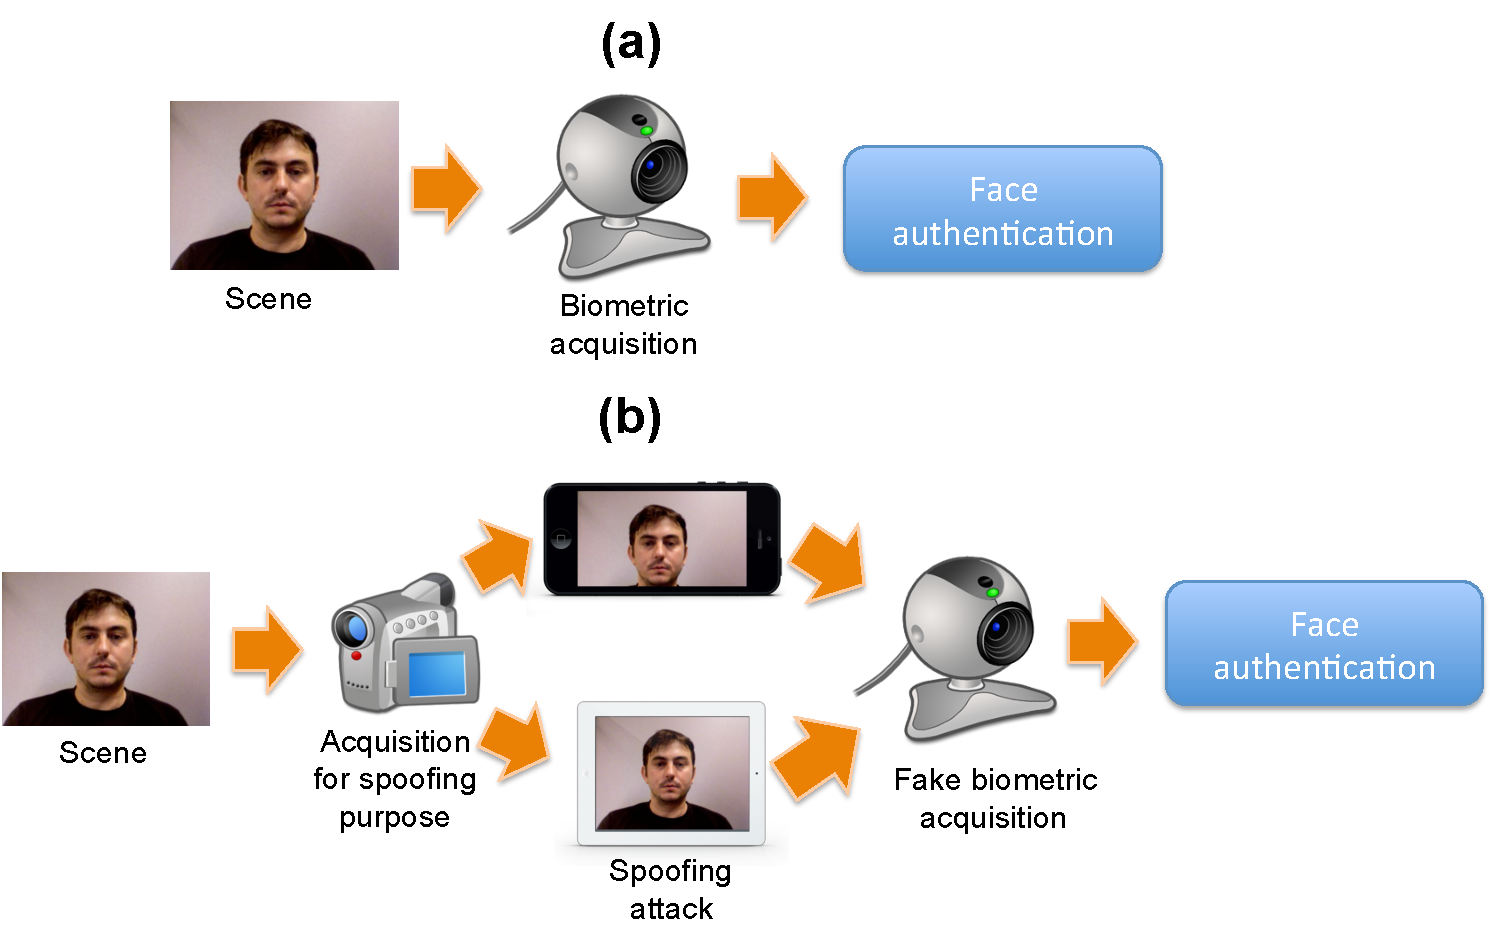
\includegraphics [width=14cm] {images/flow_spoofing.pdf}
\caption[Biometric data flow in a face authentication system]{Biometric data flow in a face authentication system (a) Biometric data flow in a real access (b) Biometric data flow in a spoofing attack} \label{fig:flow_spoofing}
\end{center}
\end{figure}

The countermeasures against spoofing attempts in face recognition can be macro classified in countermeasures that depend and do not depend on user collaboration. In countermeasures that depends on user collaboration, the user is challenged to interact to the face authentication system. For example, researchers from google are studying a way to unlock the android phones based on facial expressions\footnote{\url{http://www.bbc.co.uk/news/technology-22790221}}. As can be observed in Figure \ref{fig:google_unlock}, this strategy can be fun in the beginning but in some situations this can be embarrassing. On the other hand, countermeasures that do not depend on user collaboration try to solve this issue analysing the signal itself, without any awareness of the user. This type of countermeasures can be classified by the following cues:
\begin{itemize}
        \item Presence of vitality (liveness detection);
        \item Scene characteristics;
        \item Differences in image quality assessment.
\end{itemize}

\begin{figure}[!htb]
\begin{center}
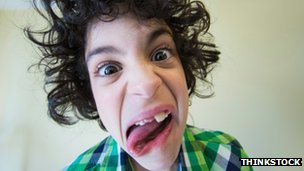
\includegraphics [width=9cm] {images/face_unlock.jpg}
\caption[New google face unlock screen]{New google face unlock screen} \label{fig:google_unlock}
\end{center}
\end{figure}

\subsection{Presence of vitality (liveness detection)}

Presence of vitality, or liveness detection, consists of the searching for features that only live faces can possess. The eye blinking is an activity that humans do constantly. A regular human blinks once every 2 or 4 seconds in order to maintain the eyes clean and wet. This frequency can vary in stress conditions and/or in a high concentration task. In that situations the interval can extend to $\sim 20$ seconds. However, does't matter in what condition the person is, the eye blink will always occur. Following that fact, \cite{pan2007eyeblink} propose a countermeasure measuring the eye blinking using Hidden Markov Models (HMM) mapping the state of eyes open and closed. Experiments carried out using a database created by the authors and freely available for download\footnote{\url{http://www.cs.zju.edu.cn/~gpan/database/db\_blink.html}}, shown an accuracy of 95.7\% .

Supported by the hypothesis that live faces present uncorrelated motion pattens in some parts of the face and the attacks do not, \cite{kollreider2009non} developed a countermeasure based on optical flow field to explore such cue. As a reference to the algorithm, were selected the center of the face an the region of the ears, as can be observed in Figure \ref{img_kollreider}.

\begin{figure}[!htb]
\begin{center}
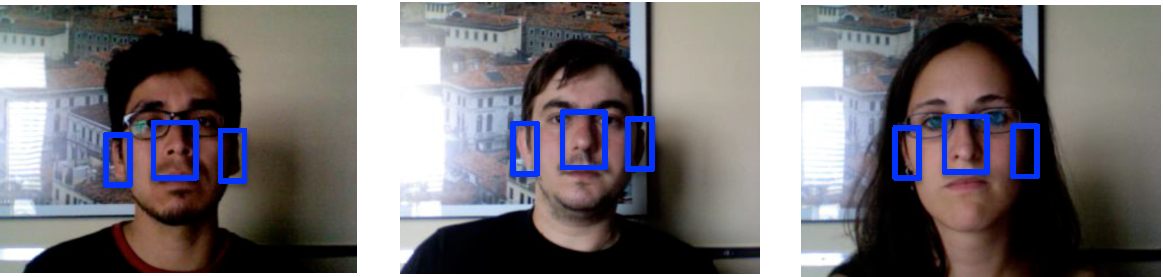
\includegraphics [width=14cm] {images/kollreider.pdf}
\caption[Face regions selection]{Face regions selection. Input for the algorithm \cite{kollreider2009non} } \label{img_kollreider}
\end{center}
\end{figure}


The strategy of the countermeasure can be summarized as follows:
\begin{enumerate}
        \item Detect the face region;
        \item Delimitate the region of the face center and the ears (Figure \ref{img_kollreider});  
        \item Determine if the face region is moving more horizontally or more vertically analysing the optical flow velocities;
        \item Compute the ratio between the velocities of the delimited areas of the face center and the ears;
        \item The spoof is detected if the aforementioned ratio was bigger than a threshold $\alpha$.
\end{enumerate}

The performance was evaluated using an adaptation of the XM2VTS database. The real accesses were videos from XM2VTS database\footnote{\url{http://www.ee.surrey.ac.uk/CVSSP/xm2vtsdb/}} and the attacks were generated with printed photographs from the same database. With this database, which was not made public, an $EER=0.5\%$ (Equal Error Rate) was achieved.

%EULERIAN.

\subsection{Scene}
\label{sec:scene_cues}

Countermeasures that search scene features analyse the relationship of the face in the scene.

The countermeasure proposed in \cite{AnjosIJCB2011}\footnote{\url{http://pypi.python.org/pypi/antispoofing.motion/}} measures the relative motion difference between the face and the background. The authors focused on simple differences of intensities in successive frames. The motion accumulated between this difference ($M_D$), for a given a Region-of-Interest (RoI) and its respective background, is computed using the following equation:

\begin{equation}
M_D  = \frac{1}{S_D} \sum_{(x,y) \in D} |I_t(D) - I_{t-1}(D)|,
\label{eq:motion}
\end{equation}
where $D$ is the RoI, $S_D$ is the area of the RoI and $I_t$ is the intensity of a pixel.

To input the motion coefficient into a classifier, 5 parameters are measured for every window of 20 frames. The parameters are: the minimum of $M_D$ in that time window, the maximum, the average, the standard deviation and the ratio $R$ between the spectral sum for all non-DC components and DC component itself taken as base the $N$-point Fourier transform of the signal (see Equation \ref{eq:motionR}). These 10 parameters (five for the face and five for the background) are fed into a Multi-layer Perceptron (MLP) classifier with 5 neurons in the hidden layer which is trained to detect spoofing attacks. This countermeasure was evaluated using the photograph attacks subset of the Replay Attack Database\cite{ChingovskaBIOSIG2012} and achieved an $HTER=9\%$ (Half Total Error Rate).

%\vspace{-2mm}
\begin{equation}
R = \frac{\sum_{i=1}^{N}|FFT_i|}{|FFT_0|}
\label{eq:motionR}
\end{equation}

%OPTICAL FLOW

\subsection{Differences in image quality assessment}
\label{sec:quality_assessment}

Countermeasures based on differences in image quality assessment rely on the presence of artifacts intrinsically present at the attack media. Such remarkable properties can be originated from media quality issues or differences in reflectance properties of the object exposed to the camera.

Compared to real faces, attack medias have different reflexive patterns. Supported by that assumption, \cite{ChingovskaBIOSIG2012} and \cite{maatta2011face}, explored the $LBP$ (Local Binary Patterns) texture descriptor analysing single frames. In this countermeasure the detected faces (see Figure \ref{fig:block-diagram}) are geometric normalized to $64 \times 64$ pixels. The $LBP$ features are extracted from the whole face region and histogrammed. The histograms for each frame are fed into a binary classifier which can be trained to detect spoofing attacks. 

\begin{figure}[!htb]
\begin{center}
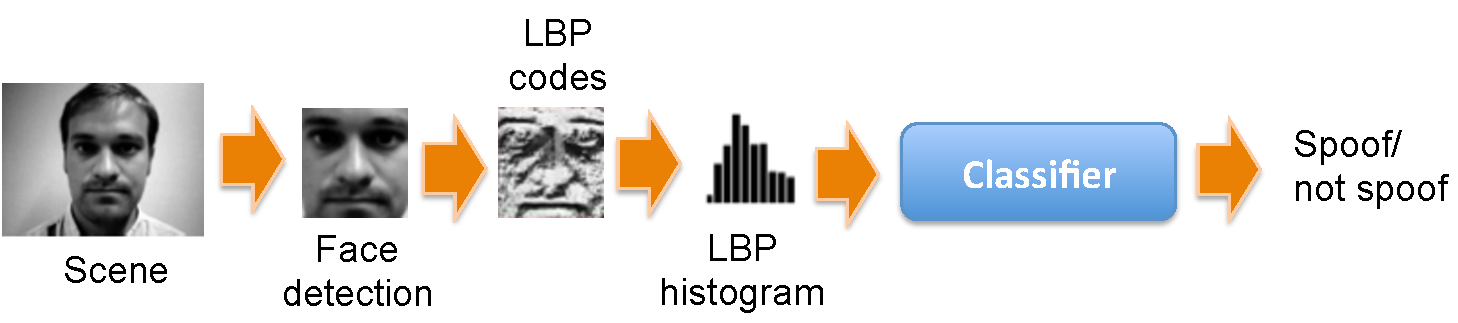
\includegraphics [width=15cm] {images/lbp_flow.pdf}
\caption[Block diagram of the countermeasure based on LBP]{Block diagram of the countermeasure based on LBP} \label{fig:block-diagram}
\end{center}
\end{figure}

The Table \ref{tb_LBP-Countermeasure} shows the reported performance, in $HTER$ terms, in the three databases; the Replay Attack Database, the CASIA FASD and the NUAA Database using the $SVM$ (Support Vector Machines) and $LDA$ (Linear Discriminant Analysis) as binary classifiers. In the test set, it can be observed a performance between $\sim15\%$ and $\sim20\%$ in the three databases. However, comparing the performance in the development set (used to tune the hyper-parameters) and in the test set of the NUAA database suggest a low generalization capability.  


\begin{table}[ht]
\caption{Performance in $HTER(\%)$ terms of the LBP countermeasure in three face spofing databases.}
\begin{center}
  \begin{tabular}{ c | c c | c c | c c | }

     \cline{2-7}    
     & \multicolumn{2}{c|}{\textbf{Replay Attack}} & \multicolumn{2}{c|}{\textbf{NUAA}}  & \multicolumn{2}{c|}{\textbf{CASIA-FASD}} \\      \cline{2-7}
     
     & dev set & test set & dev set & test set & dev set & test set \\ \hline

     \multicolumn{1}{ |c| }{$LBP_{8,1}^{u2}  + LDA $}& 19,60 & 17,17 & 0,06 & 18,32 & 17,08 & 21,01 \\ \hline
     \multicolumn{1}{ |c| }{$LBP_{8,1}^{u2}  + SVM$}& 14,84 & 15,16 & 0,11 & 19,03 & 16,00 & 18,17 \\ \hline

  \end{tabular}
\end{center}
\label{tb_LBP-Countermeasure}
\end{table}

Supported by the assumption that images/videos used in attacks concentrates information in some specifics frequency bands, \cite{zhangface} propose a countermeasure based on Difference of Gaussians filters (DoG).

As can be observed in the block diagram in Figure \ref{img:flow_DoG}, four sequences of DoG filters are applied in the image. Each the gaussian kernel has the size $3\times 3$ an it parameters are:
\begin{itemize}
  \item $\sigma_1=0,5$ e $\sigma_2=1$;
  \item $\sigma_1=1$ e $\sigma_2=1,5$;
  \item $\sigma_1=1,5$ e $\sigma_2=2$;
  \item $\sigma_1=1$ e $\sigma_2=2$.
\end{itemize}


\begin{figure}[!htb]
\begin{center}
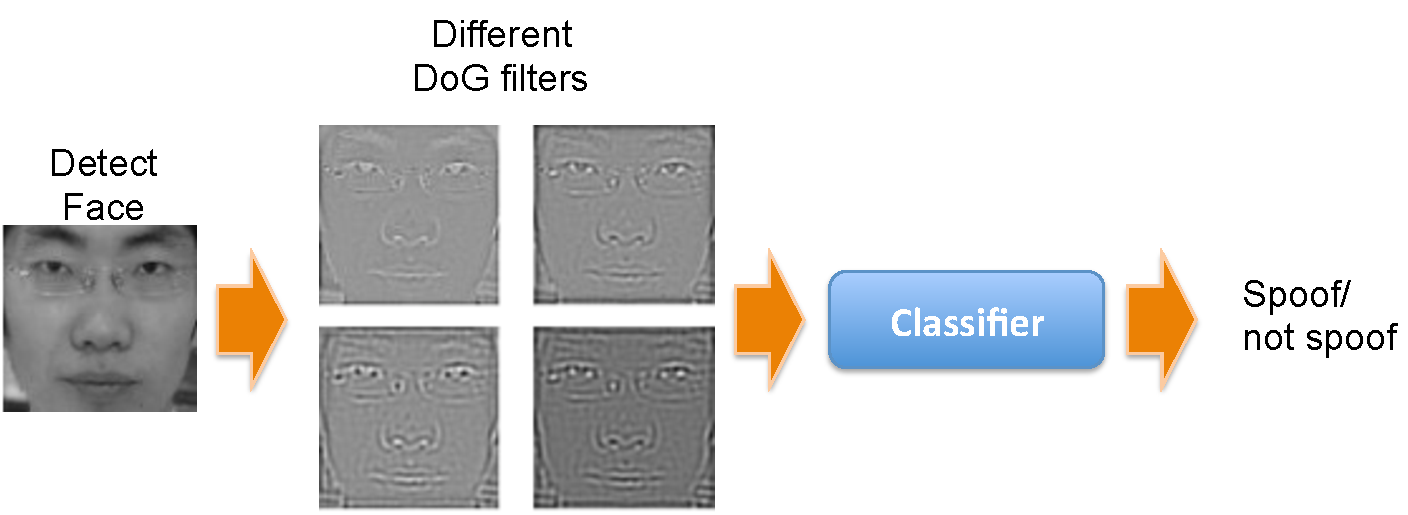
\includegraphics [width=15cm] {images/flow_DoG.pdf}
\caption{Block diagram of the DoG countermeasure} \label{img:flow_DoG}
\end{center}
\end{figure}

After of the sequence of filters, the images are geometric normalized to $128\times 128$ pixels and these data fed into a $SVM$ classifier. Evaluated using a the CASIA FASD, the countermeasure achieved an $EER$ of $17\%$. With these image dimensions, the feature vector of this countermeasure have dimensionality 65,536. The training step of the $SVM$ with this dimensionality could take several weeks. 



Li et al. \cite{li2004live} hypothesize that fraudulent photographs have less high frequency components than real ones. To test the hypothesis, a small database was built with 4 identities containing both real access and printed photo attacks. With this private database (which was not made public), an accuracy of $100\%$ was achieved. 

In order to detect noise patterns in spoofing attacks, \cite{davideo} developed a countermeasure analysing videos combining several elements. First, each frame in a frame sequence is filtered using a gaussian filter followed by a median filter. These filtered images are subtracted by the original ones. The result of this subtraction is so called "residual image". This residual image is analysed in the frequency domain using a 2D Fourier transform. All processed frames in the videos are combined using the Visual Rhythm technique\cite{zhang1995video}. This technique, generates one image with a combination of all frames ending the preprocessing steps. 

A texture description using Gray Level Co-ocurrency matrix (GLMC) was applied in the Visual Rhythm image. With the co-ocurrence matrix, 12 measures are extracted to fed into a binary classifier that will detect attacks. The classifiers evaluated was the $PLS$ (Partial Least Squares) and the $SVM$. With a database combining the photograph subset of the Replay Attack Database and a database created by the author (which was not made public), an AUC (Area Under the Curve) of $\sim100\%$ was achieved.

%%%%%%%%%%%%%%%%%%%
%%%%%%%%%%%%%%%%%%%
% Databases
%%%%%%%%%%%%%%%%%%%
%%%%%%%%%%%%%%%%%%%
\section{Face Spoofing Databases}
\label{sec:Databases}

In this section, we give an overview of the only three freely available face spoofing databases, the NUAA face antispoofing database, the Replay Attack Database and the CASIA Face Anti-Spoofing Database \cite{zhangface}, consisting of real access attempts and several fake face attacks of different natures under varying conditions. 

%Instead of still images, both datasets contain short video recordings which makes them suitable for evaluating countermeasures that exploit also temporal information.

\subsection{NUAA}
\label{sec_nuaa}

The NUAA face spoofing database\footnote{\url{http://parnec.nuaa.edu.cn/xtan/data/NuaaImposterdb.html}} \cite{tan2010face} consists of images of real accesses and attacks made with printed photographs. Emulating a scenario of access in a regular notebook, this database has images of 15 users splited in 3 section spaced in two weeks. Each section has 4 screenshots per user in different illumination conditions. Figure \ref{fig:nuaa} has some examples of this database.

%Constru�da para estudar o cen�rio de ataques utilizando fotografias impressas em papel, a base de dados NUAA\footnote{http://parnec.nuaa.edu.cn/xtan/data/NuaaImposterdb.html} consiste de capturas fotogr�ficas de pessoas em frente � c�mera de um \emph{notebook} e de ataques feitos � mesma c�mera com fotos impressas de alta qualidade destas mesmas pessoas. A base de dados possui grava��es de 15 pessoas distintas divididas em 3 se��es espa�adas em duas semanas e cada se��o possui quatro grava��es por pessoa com condi��es de ilumina��o distintas. Na Figura~\ref{fig:nuaa} s�o apresentados exemplos dessa base de dados.

\begin{figure}[!htb]
\begin{center}
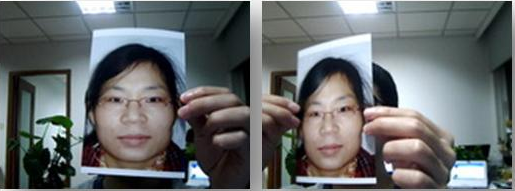
\includegraphics [width=7.5cm] {images/NUAA.png}
\caption{Printed photo attacks of the NUAA database}
\label{fig:nuaa}
\end{center}
\end{figure}


\subsection{Replay Attack Database}
\label{sec_replay}

The Replay Attack Database\footnote{\url{http://www.idiap.ch/dataset/replayattack}} \cite{ChingovskaBIOSIG2012} consists of short video ($\sim$10s) recordings of both real-access and attack attempts to 50 different identities using a laptop. It contains 1200 videos (200 real-access and 1000 attacks) and the attacks were taken in three different scenarios with two different illumination and support conditions. The scenarios of attack include:

\begin{enumerate}
        \item \textbf{print}: the attacker displays hard copies of high resolution photographs printed on A4 paper;
        \item \textbf{mobile}: the attacker displays photos and videos taken with an iPhone 3GS using the phone screen;
        \item \textbf{highdef}: The attacker displays high resolution photos and videos using an iPad screen with resolution 1024$\times$768.
\end{enumerate}
The illumination conditions include:
\begin{enumerate}
        \item \textbf{controlled}: the background of the scene is uniform and the light of a fluorescent lamp illuminates the scene;
        \item \textbf{adverse}: the background of the scene is non uniform and the day-light illuminates the scene.
\end{enumerate}
The support conditions include:
\begin{enumerate}
        \item \textbf{hand-based}: the attacker holds the attack media using his own hands;
        \item \textbf{fixed}: the attacker sets the attack device in a fixed support so it does not move during the spoofing attempt.
\end{enumerate}
Figure. \ref{fig:Database} show some examples of real accesses and attacks in different scenarios. In the top row, samples from controlled scenario. In the bottom row, samples from adverse scenario. Columns from left to right show examples of real access, printed photograph, mobile phone and tablet attacks.

\begin{figure}[!htb]
\begin{center}
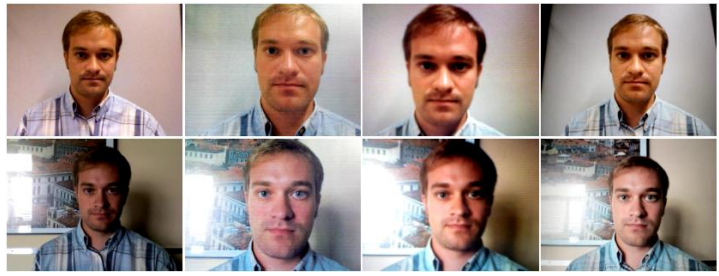
\includegraphics [width=10cm] {images/Replay_database.png}
\caption[Some frames of real access and spoofing attempts]{Some frames of real access and spoofing attempts (courtesy of \cite{ChingovskaBIOSIG2012}).} \label{fig:Database}
\end{center}
\end{figure}

The Replay Attack Database provides a protocol for objectively evaluate a given countermeasure. Such protocol defines three non-overlapping partitions for training, development (tuning) and testing countermeasures. The training set should be used to train the countermeasure, the development set is used to tune the countermeasure and to estimate a threshold value to be used in the test set. The test set must be used only to report results. As performance measurement, the protocol advises the use of Half Total Error Rate (HTER)(Equation \ref{eq:HTER}).

\begin{equation}
\label{eq:HTER}
HTER=\frac{FAR(\tau,D)+ FRR(\tau,D)} {2} ,
\end{equation}
where $\tau$ is the decision threshold, $D$ is the dataset, FAR is the False Acceptance Rate and FRR is the False Rejection Rate. In this protocol, the value of $\tau$ is estimated on the Equal Error Rate (EER) using the development set.

\begin{table}
   \label{tb_Database}
   \caption{Number of videos in each subset. Numbers displayed as sums indicate the amount of hand-based and fixed support attack available in each subset.}
   \begin{center}
     \begin{tabular}{ | l | c | c | c || c | }
      \hline
       \textbf{Type} & \textbf{Train} & \textbf{Devel.} & \textbf{Test} & \textbf{Total}\\ \hline
       Real-access & 60 & 60 & 80 & 200 \\ \hline
       Print-attack & 30+30 & 30+30 & 40+40  & 100+100\\ \hline
       Mobile-attack & 60+60 & 60+60 & 80+80 & 200+200\\ \hline
       Highdef-attack & 60+60 & 60+60 & 80+80 & 200+200\\ \hline \hline
       \textbf{Tota}l & 360 & 360 & 480 & 1200\\
       \hline
     \end{tabular}
   \end{center}
\end{table}


\subsection{CASIA Face Anti-Spoofing Database}
\label{sec_casia}


The CASIA Face Anti-Spoofing Database (CASIA FASD)\footnote{\url{http://www.cbsr.ia.ac.cn/english/FaceAntiSpoofDatabases.asp}} \cite{zhangface} contains short videos of 50 real clients and the corresponding fake faces were captured with high quality from the original ones. The database has a variety kind of attack. This variety is achieved by introducing three imaging qualities (low, normal and high) and three fake face attacks which include warped photo, cut photo (eyeblink) and video attacks. Examples from the database can be seen in Figure \ref{fig:casia_db}. Altogether the database consists of 600 video clips and the subjects are divided into subsets for training and testing (240 and 360, respectively). Results of a baseline system are also provided along the database for fair comparison. The baseline system considers the high frequency information in the facial region using multiple DoG features and SVM classifier and is inspired by the work of Tan {\em et  al.}~\cite{tan2010face}. 

Since the main purpose of the database is to investigate the possible effects of different fake face types and imaging qualities, the test protocol consists of seven scenarios in which particular train and test samples are to be used. The quality test considers the three imaging qualities separately, low (1), normal (2) and high quality (3), and evaluates  the overall spoofing detection performance under variety of attacks at the given imaging quality. Similarly, the fake face test assesses how robust the anti-spoofing measure is to specific fake face attacks, warped photo (4), cut photo (5) and video attacks (6), regardless of the imaging quality. In the overall test (7), all data is used to give a more general evaluation. The results of each scenario are reported as Detection Error Tradeoff (DET) curves and equal error rates (EER), which is the point where false acceptance rate (FAR) equals false rejection rate (FRR) on the DET curve.

\begin{figure}[!btb]
\begin{center}
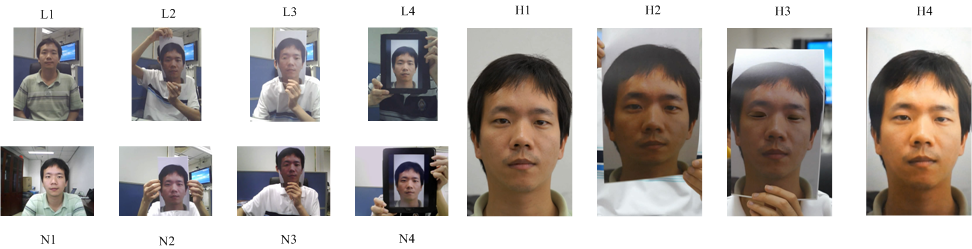
\includegraphics [width=1.0\linewidth] {images/casia_db.png}
\caption[Example images of real accesses and the corresponding spoofing attempts]{Example images of real accesses and the corresponding spoofing attempts (courtesy of \cite{zhangface})} 
\label{fig:casia_db}
\end{center}
\end{figure}


%%%%%%%%%%%%%%%%%%%
%%%%%%%%%%%%%%%%%%%
% Final Remarks
%%%%%%%%%%%%%%%%%%%
%%%%%%%%%%%%%%%%%%%
\section{Final Remarks}
\label{sec:final_remarks}

It was not until very recently that the problem of spoofing attacks against face biometric systems gained attention of the research community. This can be attested by the gradually increasing number of publicly available databases \cite{tan2010face,zhangface,ChingovskaBIOSIG2012} and the recently two contests organized \cite{ChakkaIJCB2011,Chingovska_ICB2013_2013}. With that efforts, a number of countermeasures were recently published and we presented the main of them in this chapter.

Most of the countermeasures presented in this chapter were evaluated using different metrics and in some cases in private databases, making the comparison of them a hard task. Just a few of them have source code available, making this task even worse. Additionally, the countermeasures recently published focuses only in the performance analysis in one database. The extension to more databases and the analysis of possible database bias in these countermeasures are overlooked. 

%This masters dissertation focuses 


%In this chapter were exposed how it is possible to spoof biometric systems focusing in the face biometrics, the main issue of this masters project. 

%The research community gave more attention in this kind of research mainly in the last three years. We can quote two evidences of this. The first one, two contest were organized in the last two years calling researchers to develop countermeasures. The second one; three databases were freely released in the last three years. The Section \ref{SpoofingAttacksFaceRec} shown that the most of the countermeasures presented in the literature were evaluated using different metrics and in some cases in private databases, make the work of comparison a hard task. 

